%--------------------------------------------------------------
% thesis.tex 
%--------------------------------------------------------------
% Corso di Laurea in Informatica 
% http://if.dsi.unifi.it/
% @Facolt\`a di Scienze Matematiche, Fisiche e Naturali
% @Universit\`a degli Studi di Firenze
%--------------------------------------------------------------
% - template for the main file of Informatica@Unifi Thesis 
% - based on Classic Thesis Style Copyright (C) 2008 
%   Andr\'e Miede http://www.miede.de   
%--------------------------------------------------------------
\documentclass[twoside,openright,titlepage,fleqn,
	headinclude,12pt,a4paper,BCOR=5mm,footinclude]{scrbook}
%--------------------------------------------------------------
\newcommand{\myItalianTitle}{Titolo italiano\xspace}
\newcommand{\myEnglishTitle}{Titolo inglese\xspace}
% use the right myDegree option
\newcommand{\myDegree}{Corso di Laurea in Informatica\xspace}
%\newcommand{\myDegree}{
	%Corso di Laurea Specialistica in Scienze e Tecnologie 
	%dell'Informazione\xspace}
\newcommand{\myName}{Nome Candidato\xspace}
\newcommand{\myProf}{Relatore\xspace}
\newcommand{\myOtherProf}{Correlatore\xspace}
\newcommand{\mySupervisor}{Nome Cognome\xspace}
\newcommand{\myFaculty}{
	Scuola di Scienze Matematiche, Fisiche e Naturali\xspace}
\newcommand{\myUni}{\protect{
	Universit\`a degli Studi di Firenze}\xspace}
\newcommand{\myLocation}{Firenze\xspace}
\newcommand{\myTime}{Anno Accademico 2014-2015\xspace}
\newcommand{\myVersion}{Version 0.1\xspace}
%--------------------------------------------------------------
\usepackage[italian]{babel}
\usepackage[utf8]{inputenc} %\usepackage[latin1]{inputenc}
\usepackage[T1]{fontenc} 
\usepackage[scaled]{helvet} %\usepackage[default]{nome_font}
\usepackage[square,numbers]{natbib} 
\usepackage[fleqn]{amsmath}  
\usepackage{ellipsis}
\usepackage{listings}
\usepackage{subfig}
\usepackage{caption}
\usepackage{appendix}
\usepackage{siunitx}
%--------------------------------------------------------------
\usepackage{dia-classicthesis-ldpkg}
%\usepackage{classicthesis}
%--------------------------------------------------------------
% Options for classicthesis.sty:
% tocaligned eulerchapternumbers drafting linedheaders 
% listsseparated subfig nochapters beramono eulermath parts 
% minionpro pdfspacing
\usepackage[eulerchapternumbers,linedheaders,subfig,beramono,eulermath,
parts,dottedtoc]{classicthesis}
%--------------------------------------------------------------
\newlength{\abcd} % for ab..z string length calculation
% how all the floats will be aligned
\newcommand{\myfloatalign}{\centering} 
\setlength{\extrarowheight}{3pt} % increase table row height
\captionsetup{format=hang,font=small}
%--------------------------------------------------------------
% Layout setting
%--------------------------------------------------------------
\usepackage{geometry}
\geometry{
	a4paper,
	ignoremp,
	bindingoffset = 1cm, 
	textwidth     = 13.5cm,
	textheight    = 21.5cm,
	lmargin       = 3.5cm, % left margin
	tmargin       = 4cm    % top margin 
}

\lstset{
  	%frame=tb,
	language=Matlab,
  	aboveskip=3mm,
  	belowskip=3mm,
  	showstringspaces=false,
  	columns=flexible,
  	basicstyle={\small\ttfamily},
  	numbers=none,
  	breaklines=true,
  	breakatwhitespace=true,
  	tabsize=3
}
\usepackage{dirtree}
\usepackage{url}
\usepackage{float}
%--------------------------------------------------------------
\begin{document}
\frenchspacing
\raggedbottom
\pagenumbering{roman}
\pagestyle{plain}
%--------------------------------------------------------------
% Frontmatter
%--------------------------------------------------------------
%--------------------------------------------------------------
% titlepage.tex (use thesis.tex as main file)
%--------------------------------------------------------------
\begin{titlepage}
	\begin{center}
   	\large
      \hfill
      \vfill
      \begingroup
         \includegraphics[scale=0.15]{logo/LOGO}\\
%			\spacedallcaps{\myUni} \\ 
			\myFaculty \\
			\myDegree \\ 
			\vspace{0.5cm}
         \vspace{0.5cm}    
         Tesi di Laurea    
      \endgroup 
      \vfill 
      \begingroup
      	\color{Maroon}\spacedallcaps{\myItalianTitle} \\ $\ $\\
      	\spacedallcaps{\myEnglishTitle} \\ 	
	\bigskip
      \endgroup
      \spacedlowsmallcaps{\myName}
      \vfill 
      \vfill
      Relatore: \emph{\myProf}\\
      %Correlatore: \emph{Correlatore}\\
      \vfill
      \vfill
      \myTime
      \vfill                      
	\end{center}        
\end{titlepage}   
%--------------------------------------------------------------
% back titlepage
%--------------------------------------------------------------
   \newpage
	\thispagestyle{empty}
	\hfill
	\vfill
	\noindent\myName: 
	\textit{\myItalianTitle,} 
	\myDegree, \textcopyright\ \myTime
%--------------------------------------------------------------
% back titlepage end
%--------------------------------------------------------------
\pagestyle{scrheadings}
%--------------------------------------------------------------
% Mainmatter
%--------------------------------------------------------------
\pagenumbering{arabic}
% use \cleardoublepage here to avoid problems with pdfbookmark
%\include{intro} % use \myChapter command instead of \chapter
\tableofcontents
%\listoffigures
\cleardoublepage
\thispagestyle{empty}
\begin{flushright}
\null\vspace{\stretch {1}}
\emph{"Inserire citazione" \break --- Inserire autore citazione} \vspace{\stretch{2}}\null
\end{flushright}
\cleardoublepage
\chapter{Introduzione}
In questa introduzione sarà presente una prima parte che andrà a dare le conoscenze di base minime per comprendere cosa sia un sistema operativo e una piccola classificazione, dopodiché seguiranno la descrizione di alcuni concetti che sono fondamentali per comprendere il resto dell'elaborato.

\section{Cos'è un sistema operativo}
Un sistema operativo (SO) è un insieme di software che gestisce le risorse hardware e software di un sistema di elaborazione fornendo servizi agli applicativi utente.\\
In un computer quindi il sistema operativo fornisce l'unica interfaccia diretta con l'hardware e in quanto tale ha un accesso esclusivo con il massimo dei privilegi detto \textit{kernel mode}. Questo comporta che una vulnerabilità all'interno del sistema operativo può portare a gravi conseguenze per l'integrità e la sicurezza del sistema, inoltre qualche malintenzionato potrebbe approfittare di questo bug per trarne profitto.
Uno degli obiettivi principali di un SO è quindi quello di garantire la sicurezza, ulteriore scopo è l'efficienza: un buon sistema operativo deve saper sfruttare al meglio tutte le risorse che ha a disposizione, dalla gestione della memoria per sfruttare al meglio lo spazio alla schedulazione dei processi per ottimizzare i tempi di esecuzione. Come ultimo obiettivo, ma non per questo meno rilevante, deve rendere il più semplice possibile l'utilizzo del dispositivo su cui è installato.
Dalla definizione di SO data a inizio capitolo possiamo isolare una specifica parte di codice che è quella che permette al software di interfacciarsi con l'hardware, quindi l'accesso e la gestione delle risorse di un dispositivo, questa specifica parte si chiama \textit{kernel} che come suggerisci il nome (nocciolo dall'inglese) rappresenta la parte centrale di un sistema operativo su cui tutto il resto si appoggia.
\newpage

\section{Microkernel e kernel monolitici}
Esistono vari modelli strutturali per i sistemi operativi: monolitici, modulari, a livelli, microkernel ed ibridi, ad oggi i più diffusi sono gli ibridi, che combinano i vari modelli tra di loro, ma che in gran parte si basano su sistemi monolitici i quali consistono di un unico file binario statico al cui interno sono definite tutte le funzionalità del kernel e che viene eseguito in un unico spazio di indirizzi, questo comporta dei vantaggi: 
\begin{itemize}
	\item[-] efficienza $\rightarrow$ motivo principale per cui la maggior parte dei sistemi operativi ancora si basano su kernel in gran parte monolitici, lavorando nello stesso spazio di indirizzi e gestendo tutto attraverso chiamate a procedura il SO risulterà molto reattivo e performante
	\item[-] semplicità $\rightarrow$ in quanto non ha una vera e  propria strutturazione ma il codice è tutto in un unico file binario risulta chiaramente più semplice da progettare anche se poi l'implementazione risulta difficile
\end{itemize} 
d'altra parte ha anche degli svantaggi: 
\begin{itemize}
	\item[-] inserimento di un nuovo servizio $\rightarrow$ questo richiede la ricompilazione del kernel, quindi non permette l'inserimento di un nuovo servizio a runtime (problema risolto nei modelli ibridi)
	\item[-] dimensione $\rightarrow$ dovendo gestire tutte le principali funzionalità del sistema operativo il kernel sarà composto da milioni di righe di codice sorgente (MSLOC - linux ha circa 20MSLOC) e questo porta direttamente al successivo grosso svantaggio
	\item[-] sicurezza $\rightarrow$ maggiore è il numero di righe di codice maggiore sarà il numero di possibili bug, essendo tutto il codice eseguito nello stesso spazio di indirizzi un bug rischia di far 	bloccare l'intero sistema anche se il problema è molto piccolo e isolato a una minima funzione del kernel.
\end{itemize}
All'estremo opposto troviamo i \textit{microkernel} che sono composti da un kernel ridotto al minimo indispensabile, che comprende la gestione della memoria, dei processi e della CPU, le comunicazioni tra processi (IPC) e l'hardware di basso livello, mentre tutto il resto deve essere gestito da server (deamon) che operano sopra al kernel, quindi in spazi di indirizzi separati.\\ I microkernel sono spesso usati in sistemi embedded in applicazioni mission critical di automazione robotica o di medicina, a causa del fatto che i componenti del sistema risiedono in aree di memoria separate, private e protette.\\
Anche questo modello ha dei vantaggi:
\begin{itemize}
	\item[-] flessibilità $\rightarrow$ l'inserimento di un nuovo servizio avviene al di sopra del kernel quindi in qualsiasi momento è possibili aggiungere o togliere servizi senza dover modificare il kernel.
	\item[-] sicurezza $\rightarrow$ minore quantità di codice eseguita in kernel mode (quindi minore quantità di bug e minore superficie attaccabile) maggiore è la sicurezza del sistema, inoltre i servizi sono lavorano in uno spazio di indirizzi differente da quello del kernel di conseguenza se un server (su cui viene eseguito un servizio) smette di funzionare tutto il resto del sistema continua a funzionare normalmente e si potrà procedere a riavviare quel singolo servizio
	\item[-] semplicità $\rightarrow$ essendo il codice composto da giusto qualche decina di migliaia di righe di codice (KSLOC) risulta molto più facile da scrivere
\end{itemize}
e dall'altro lato ha un grande svantaggio:
\begin{itemize}
	\item[-] efficienza $\rightarrow$ dato che ogni servizio gira a livello utente l'utilizzo di uno qualsiasi di questi richiede il ricorso a chiamate di sistema che rallentano fortemente l'esecuzione di ogni operazione, motivo principale per cui ancora oggi i sistemi operativi si basano in gran parte su sistemi monolitici.
\end{itemize}

\begin{figure}[h]
  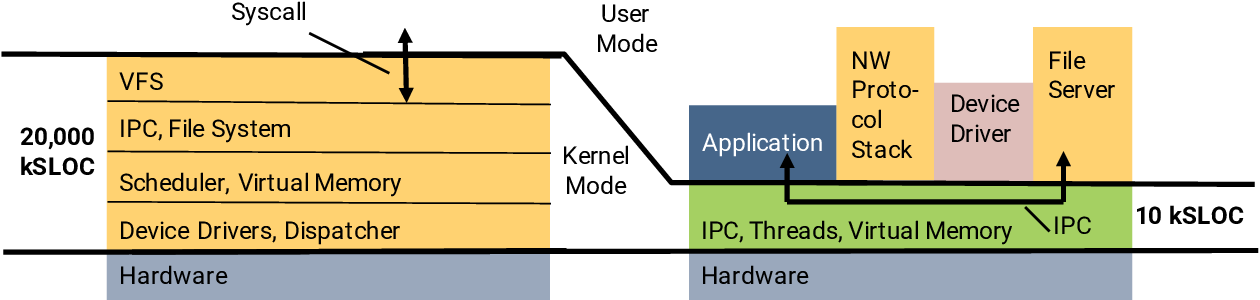
\includegraphics[width=\linewidth]{img/MonolithicVSmicrokernel.png}
  \caption{Kernel monolitici (sinistra) VS microkernel (destra)}
  \label{fig:MonolithicVSmicrokernel}
\end{figure}
\newpage

\section{Scheduling}
Proseguendo la lettura verrà nominato lo scheduling: solitamente con il solo termine scheduling si intende quello a breve termine della CPU, cioè la funzionalità che determina quale tra i processi (thread) in attesa della CPU la otterranno, ci sono vari metodi che si differenziano per modalità e prestazioni, gli algoritmi che traducono questi metodi si chiamano politiche di scheduling.
Una particolare politica di scheduling rilevante per questo testo è Round Robin o scheduling circolare: consiste nel determinare una quantità di tempo (time slice) nella quale il processo ottiene la CPU al termine del quale il processo viene interrotto e inserito infondo alla lista dei processi in attesa, in questo modo tutti i processi ottengono la CPU per al più un tempo massimo stabilito ed è anche possibile stabilire un tempo massimo di attesa che un processo dovrà attendere in base a quanti processi lo precedono.

\section{Hypervisor}
Un \textit{hypervisor}, chiamato anche virtual machine monitor (VMM), è un tipo di sotware/firmware che permette di creare ed eseguire macchine virtuali. Un computer sul quale un hypervisor esegue una o più macchine virtuali prende il nome di host machine mentre le singole macchina virtuali prenderanno il nome di guest machine, su ognuna di queste è possibile far girare un sistema operativo diverso che eseguirà la maggior parte delle istruzioni direttamente sulle risorse hardware virtualizzate rese disponibili dall'hypervisor.
\include{Chapters/sel4}
\chapter{Impostazione di seL4}
Come primo approccio per arrivare alla scrittura di questa tesi ho innanzitutto fatto una ricerca sulla letteratura che si trova disponibile riguardo a seL4, nonostante sia poca e principalmente fornita da Trustworthy (TS) stesso comunque sufficiente per avere una conoscenza abbastanza approfondita del microkernel.\\
SeL4 è un sistema open-source dunque lo step successivo è stato quello di scaricare seL4 e sperimentare con mano le funzionalità, ovviamente questo ha richiesto un approfondimento più tecnico e specifico, rispetto a quanto fatto finora, di alcuni aspetti come la gestione della memoria fisica e virtuale, l'IPC ecc. che verranno trattati in questo capitolo.

\section{Fase iniziale: prerequisiti}
Come prima cosa ho installato sul mio portatile VirtualBox in quanto come consigliato dalle guide fornite da TS sarebbe ottimale lavorare in ambiente Linux, non avendo una partizione del portatile con Linux ho inizialmente pensato di utilizzare una macchina virtuale così da lasciare inalterato il mio computer e comunque avere a disposizione un sistema operativo Linux su cui lavorare. Andando avanti con il set-up del sistema per iniziare a lavorare su seL4 però ho incontrato una prima difficoltà che è stata lo spazio: purtroppo lo spazio nel portatile non era tantissimo, la macchina virtuale, considerando il sistema operativo e l'installazione dei vari prerequisiti per poter far girare il microkernel, cominciava ad occupare molto spazio, dunque ho dovuto cercare un'alternativa; Per sopperire al problema mi sono procurato un SSD su cui sono andato a copiare la partizione creata in VirtualBox continuando la sperimentazione sul microkernel lavorando sull'SSD esterno collegato via USB.\\
Per lavorare su seL4 è necessario avere installato sul sistema dei programmi che simulino un'architettura su cui farlo girare, per fare ciò è necessario installare delle dipendenze (prerequisiti) cioè compilatori, emulatori software vari e librerie che devono essere installate affinché sia possibile utilizzare seL4.\\
Prima di tutto ho installato Google repo, così da poter clonare i repository git:
\definecolor{codegreen}{rgb}{0,0.6,0}
\definecolor{codegray}{rgb}{0.5,0.5,0.5}
\definecolor{codepurple}{rgb}{0.58,0,0.82}
\definecolor{backcolour}{rgb}{0.95,0.95,0.92}
\lstdefinestyle{mystyle}{
    backgroundcolor=\color{backcolour},   
    commentstyle=\color{codegreen},
    keywordstyle=\color{magenta},
    numberstyle=\tiny\color{codegray},
    stringstyle=\color{codepurple},
    basicstyle=\ttfamily\footnotesize,
    breakatwhitespace=false,         
    breaklines=true,                 
    captionpos=b,                    
    keepspaces=true,                  
    numbersep=5pt,                  
    showspaces=false,                
    showstringspaces=false,
    showtabs=false,                  
    tabsize=2
}

\lstset{style=mystyle}

\begin{lstlisting}[language=bash]
sudo apt-get install repo
\end{lstlisting}
build-essential, cmake, ninja, curl, python e QEMU abbreviazione di Quick EMUlator, un emulatore open-source che permette di emulare un'architettura informatica e che permette di simulare diversi sistemi operativi, in questo caso è fondamentale perchè permette l'esecuzione di seL4:
\begin{lstlisting}[language=bash]
sudo apt-get install build-essential
sudo apt-get install cmake ccache ninja-build cmake-curses-gui
sudo apt-get install libxml2-utils ncurses-dev
sudo apt-get install curl git doxygen device-tree-compiler
sudo apt-get install u-boot-tools
sudo apt-get install python3-dev python3-pip python-is-python3
sudo apt-get install protobuf-compiler python3-protobuf
sudo apt-get install qemu-system-arm qemu-system-x86 qemu-system-misc
pip3 install --user setuptools
pip3 install --user sel4-deps
\end{lstlisting}
Altro componente fondamentale è CAmkES (component architecture for microkernel-based embedded systems), un framework per realizzare velocemente sistemi multiserver affidabili basati su microkernel:
\begin{lstlisting}[language=bash]
pip3 install --user camkes-deps
curl -sSL https://get.haskellstack.org/ | sh
sudo apt-get install haskell-stack
sudo apt-get install clang gdb
sudo apt-get install libssl-dev libclang-dev libcunit1-dev libsqlite3-dev
sudo apt-get install qemu-kvm
\end{lstlisting}
Dopodiché sono passato alle dipendenze per l'installazione di Isabelle (theorem prover) che serve per la verifica automatica di sistemi software e hardware:
\begin{lstlisting}[language=bash]
sudo apt-get install \
    python3 python3-pip python3-dev \
    gcc-arm-none-eabi build-essential libxml2-utils ccache \
    ncurses-dev librsvg2-bin device-tree-compiler cmake \
    ninja-build curl zlib1g-dev texlive-fonts-recommended \
    texlive-latex-extra texlive-metapost texlive-bibtex-extra \
    mlton-compiler haskell-stack repo
\end{lstlisting}
Ancora dipendenze Python e Haskell
\begin{lstlisting}[language=bash]
pip3 install --user --upgrade pip
pip3 install --user sel4-deps

stack upgrade --binary-only
which stack # should be $HOME/.local/bin/stack
stack install cabal-install
\end{lstlisting}
Con questa serie di comandi bash il sistema operativo Linux, per la precisione Ubuntu \textcolor{red}{VERSIONE}, ha tutti i prerequisiti necessari per procedere alla configurazione.

\section{Configurazione}
Lo step successivo è stato quello di recuperare, attraverso repo, la collezione di repository necessari per la verifica di seL4; in particolare contiene il sorgente del kernel, il theorem prover Isabelle/HOL e HOL4 e lo strumento di verifica binaria.
\begin{lstlisting}[language=bash]
mkdir verification
cd verification
repo init -u https://git@github.com/seL4/verification-manifest.git
repo sync
\end{lstlisting}
A questo punto  si avrà quindi una cartella con questa struttura:
\dirtree{%
.1 verification.
.2 HOL4/.
.2 graph-refine/.
.2 isabelle/.
.2 l4v/.
.2 seL4/.
}
Il che indica che l'importazione delle repository è andata a buon fine, quindi possiamo procedere alla configurazione di Isabelle posizionandosi nella cartella \texttt{l4v}:
\begin{lstlisting}[language=bash]
mkdir -p ~/.isabelle/etc
cp -i misc/etc/settings ~/.isabelle/etc/settings
./isabelle/bin/isabelle components -a
./isabelle/bin/isabelle jedit -bf
./isabelle/bin/isabelle build -bv HOL
\end{lstlisting}
Questa serie di comandi bash daranno come risultato:
\begin{itemize}
	\item[*] la creazione di una cartella per le impostazioni utente di Isabelle.
	\item installazione delle impostazione Isabelle per L4.verified \cite{l4v} 
\end{itemize} 

create an Isabelle user settings directory.

install L4.verified Isabelle settings. These settings initialise the Isabelle installation to use the standard Isabelle contrib tools from the Munich Isabelle repository and set up paths such that multiple Isabelle repository installations can be used side by side without interfering with each other.

download contrib components from the Isabelle repository. This includes Scala, a Java JDK, PolyML, and multiple external provers. You should download these, even if you have these tools previously installed elsewhere to make sure you have the right versions. Depending on your internet connection, this may take some time.

compile and build the Isabelle PIDE jEdit interface.

build basic Isabelle images to ensure that the installation works. This may take a few minutes.
\nocite{*}
\bibliography{bibliografia}
\bibliographystyle{plainurl}
%--------------------------------------------------------------
\end{document}
%--------------------------------------------------------------
